% Created 2009-12-13 Sun 11:42
\documentclass[11pt]{article}
\usepackage[utf8]{inputenc}
\usepackage[T1]{fontenc}
\usepackage{mathpazo}
\usepackage{graphicx}
\usepackage{longtable}
\usepackage{soul}
\usepackage{hyperref}
\usepackage{fullpage}
\usepackage{color}
\usepackage{listings}


\title{Genetic Programming on IXM}
\author{Eric Schulte}
\date{13 December 2009}

\begin{document}

\maketitle


\section*{Report}
\label{sec-1}
\subsection*{Boards}
\label{sec-1.1}

quick desc. and properties relevant to GP
\subsection*{GP}
\label{sec-1.2}

implementation and how/why different from vanilla GP
\subsection*{evo co-evo}
\label{sec-1.3}
\subsection*{results}
\label{sec-1.4}
\section*{Data Analysis}
\label{sec-2}
\subsection*{basic GP parameters}
\label{sec-2.1}

just to show that mutation and crossover actually help, and to justify
the choices used in later experiments
\subsection*{GP visualization}
\label{sec-2.2}

evo-individuals and coevo-individuals

connect the gnuplot graphics to the text files of results

\begin{enumerate}
\item ingest text files
\item persist in serialized ruby structures
\item connect to group/board data structures
\item produce graphs
\end{enumerate}
\subsection*{plot fitness by time}
\label{sec-2.3}

many data points, maybe a best-fit line w/R
\subsection*{comparisons}
\label{sec-2.4}
\subsubsection*{sharing rates}
\label{sec-2.4.1}


\lstset{language=Ruby}
\begin{lstlisting}
ave_max_time = {}
[100, 1000, 10000].each do |share|
  data_s = goal2.select{|d| d.share == share}
  ave_max_time[share] = (0..9).map{ |run| data_s.sort_by{|d| d.time}.last }.
    inject(0){|a, p| a += p.time } / 4
end
\end{lstlisting}

need to clear out individuals from previous runs -- namely those
returned before the reset packet
\lstset{language=Ruby}
\begin{lstlisting}
# make sure to remove individuals from before reset packet
temp_goal2 = goal2.reject{|d| d.time < 4};
\end{lstlisting}

\lstset{language=Ruby}
\begin{lstlisting}
ave_best_score = {}
[100, 1000, 10000].each do |share|
  data_s = temp_goal2.select{|d| d.share == share}
  ave_best_score[share] = (0..9).map{|run| data_s.sort_by{|d| d.score}.first}.
    inject(0){|a, p| a += p.score } / 9
end
\end{lstlisting}

\lstset{language=Ruby}
\begin{lstlisting}
best_inds = {}
[100, 1000, 10000].each do |share|
  data_s = temp_goal2.select{|d| d.share == share}
  best_inds[share] = (0..9).map{|run| data_s.sort_by{|d| d.score}.first}.
    sort_by{|d| d.score}.first
end
\end{lstlisting}


\begin{itemize}
\item Goal 2

\begin{itemize}
\item runtime -- no runs completed
\begin{lstlisting}
irb(main):052:0> ave_max_time
ave_max_time
{10000=>1207.943955, 100=>1207.720609, 1000=>1210.959188}
\end{lstlisting}
\item score -- looks like two actually succeeded\ldots{}
\begin{lstlisting}
irb(main):096:0> ave_best_score
ave_best_score
{10000=>255.311111111111, 100=>253.433333333333, 1000=>183.966666666667}
\end{lstlisting}
\item best individuals
\end{itemize}

\end{itemize}


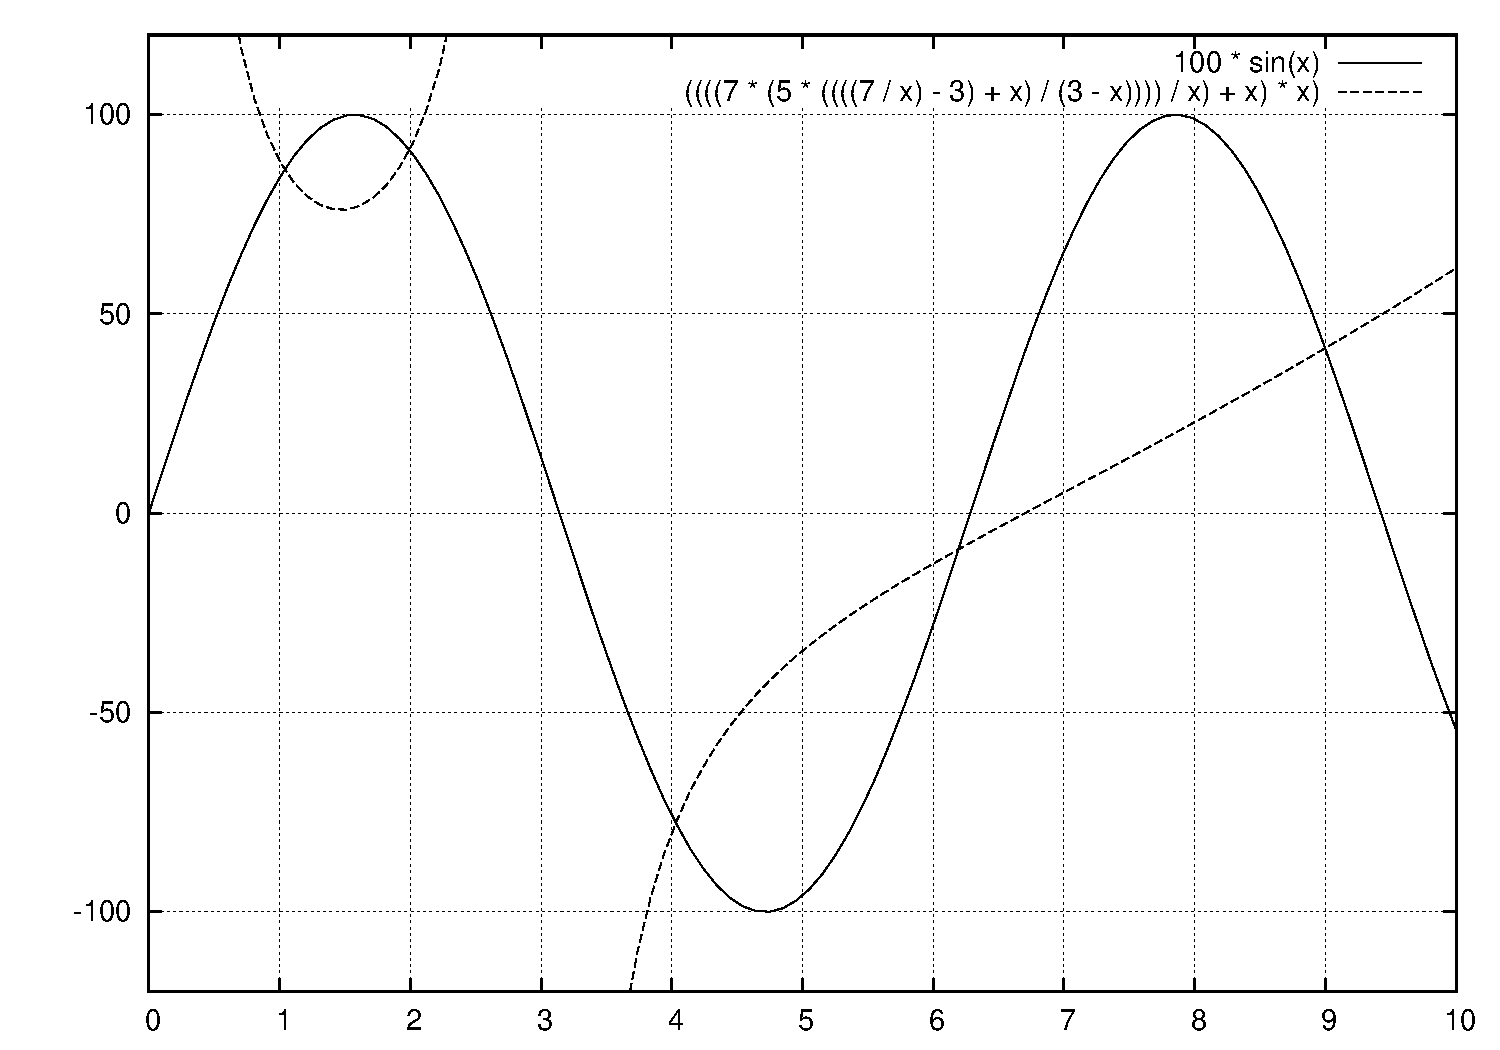
\includegraphics[width=\textwidth]{graphs/s_100_g_2_best.pdf}
    
\subsubsection*{line vs. eight}
\label{sec-2.4.2}
\subsection*{common tools}
\label{sec-2.5}
\subsubsection*{ingest}
\label{sec-2.5.1}

ingest a directories worth of run results and return a list of Datum
\lstset{language=Ruby}
\begin{lstlisting}
class Datum
  attr_accessor :share, :goal, :run, :time, :score, :path
end
def ingest(base)
  Dir.entries(base).map do |e|
    if e.match(/r_s.(\d+)_m.(\d+)_b.(\d+)_i.(\d+)_g.(\d+).(\d+)/)
      share = Integer($1)
      goal  = Integer($5)
      run   = Integer($6)
      File.read(File.join(base, e)).map do |l|
        if l.match(/^([\d\.\/-]+)\t([\d\.\/-]+)\t([frl]+)$/)
          d = Datum.new
          d.share = share
          d.goal  = goal
          d.run   = run
          d.time  = Float($1) rescue -1
          d.score = Float($2) rescue -1
          d.path  = $3
          d
        end
      end.compact
    end
  end.compact.flatten
end
\end{lstlisting}

test ingest -- works -- 512783 data points in the directory
\lstset{language=Ruby}
\begin{lstlisting}
<<ingest>>
data = ingest("./raw/15-evo-eight/");''
puts data.size
\end{lstlisting}
\begin{itemize}

\item serialize -- not plausible\\
\label{sec-2.5.1.1}%
tried YAML and sqlite3 and neither worked in a reasonable amount of
time

creating a sqlite3 table to hold this info
\lstset{language=Ruby}
\begin{lstlisting}
# create database
db = SQLite3::Database.new('raw.db')

table = "evo_eight"

# create table
db.execute("create table #{table} (share INT, goal INT, run INT, time FLOAT, score FLOAT, path STRING);")

# define keys
keys = %w{share goal run time score path}

# create a large insert statement for 1000 data points
stmt = data.map{ |d| "insert into #{table} (#{keys.join(", ")}) values (#{keys[0..-2].map{|k| d.send(k.intern) }.join(", ")}, '#{d.path}');" }

db.transaction{ |db| db.execute_batch(stmt.join("\n")) }
\end{lstlisting}

\end{itemize} % ends low level
\subsubsection*{rpn to alg}
\label{sec-2.5.2}


evo individuals are check on the (0..9) range inclusive


\begin{center}
\begin{tabular}{l}
 0757x/3-x+3x-/**x/x+x*  \\
\end{tabular}
\end{center}



\lstset{language=Ruby}
\begin{lstlisting}
operators = %W{+ - / *}
$stack = []
ind[0][0].split(//).each do |ch|
  if operators.include?(ch)
    right = $stack.pop or "1"
    left = $stack.pop or "1"
    $stack.push("(#{left} #{ch} #{right})")
  else
    $stack.push(ch)
  end
end
puts $stack.pop
\end{lstlisting}

\begin{verbatim}
 ((((7 * (5 * ((((7 / x) - 3) + x) / (3 - x)))) / x) + x) * x)
\end{verbatim}


\end{document}